
\begin{multicols}{2}
$ACDF$ est un rectangle et $BCDE$ est un carré.\\
 
$M$ est un point du segment $[AF]$ et les droites $(MK)$ et $(CD)$
sont perpendiculaires.\\
 
Le point $M$ peut se déplacer sur le segment $[AF]$.

\medskip 

Que peut-on dire
de la longueur $IJ$ en fonction de la position du point $M$ sur le
segment $[AF]$ ?\\

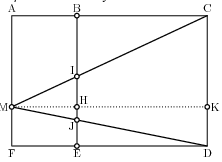
\includegraphics[scale=1]{TR-exo23.png} 

\end{multicols}

